\chapter{Deneysel Düzenek}
Insanlik bu zamana kendini ve cevresini anlamak istemiştir. Çevresinde olan olayların temelde neden olduğunu merak edip altindaki sebebi açıklama isteği duymuştur. Bunlardan biri çevremizde gördüğümüz şey nedir ? ve bu merakın sonucu insanlığın sorduğu en güzel sorulardan biri en küçük nedir sorusudur. Bu soruya yüzyıllardır çeşitli cevaplar verilmiştir gerek felsefi gerek bilimsel. Bilimsel olarak ele aldığımızda insalık en küçüğe bir isim vermiştir ve buna atom (atomus \footnote{Atomus sözcüğünü ortaya atan ilk kişi MÖ 440'lı yıllarda yaşamış Demokritos'tur.}) demiştir. Daha sonrakı tarihsel kısımda ise atomun çekirdeğinin keşfi 1911 yılında Ernest Rutherford tarafından 2 atom inceliğinde altın bir folyo üzerine gönderdiği alfa lar ile yaptı. Bilimin en küçüğü arama yöntemi zaman geçtikçe değisti. Çekirdiği oluşturan protonlar ve nötronlar keşfedildi. 1964 yılında Murray Gell-Mann ve George Zweig tarafından birbirlerinden bağımsız olarak quark modelini ortaya attılar. Böylece tarihin en küçüğü arama mücadelesi ayni kalirken, küçüğü bulma yolundaki yöntemleri değisti. Şu anda en küçükleri arama aracı olarak hızlandırıcıları kullanıyoruz.\\
\begin{figure}[!htpb]
  \centering
  \begin{minipage}[b]{0.4\textwidth}
    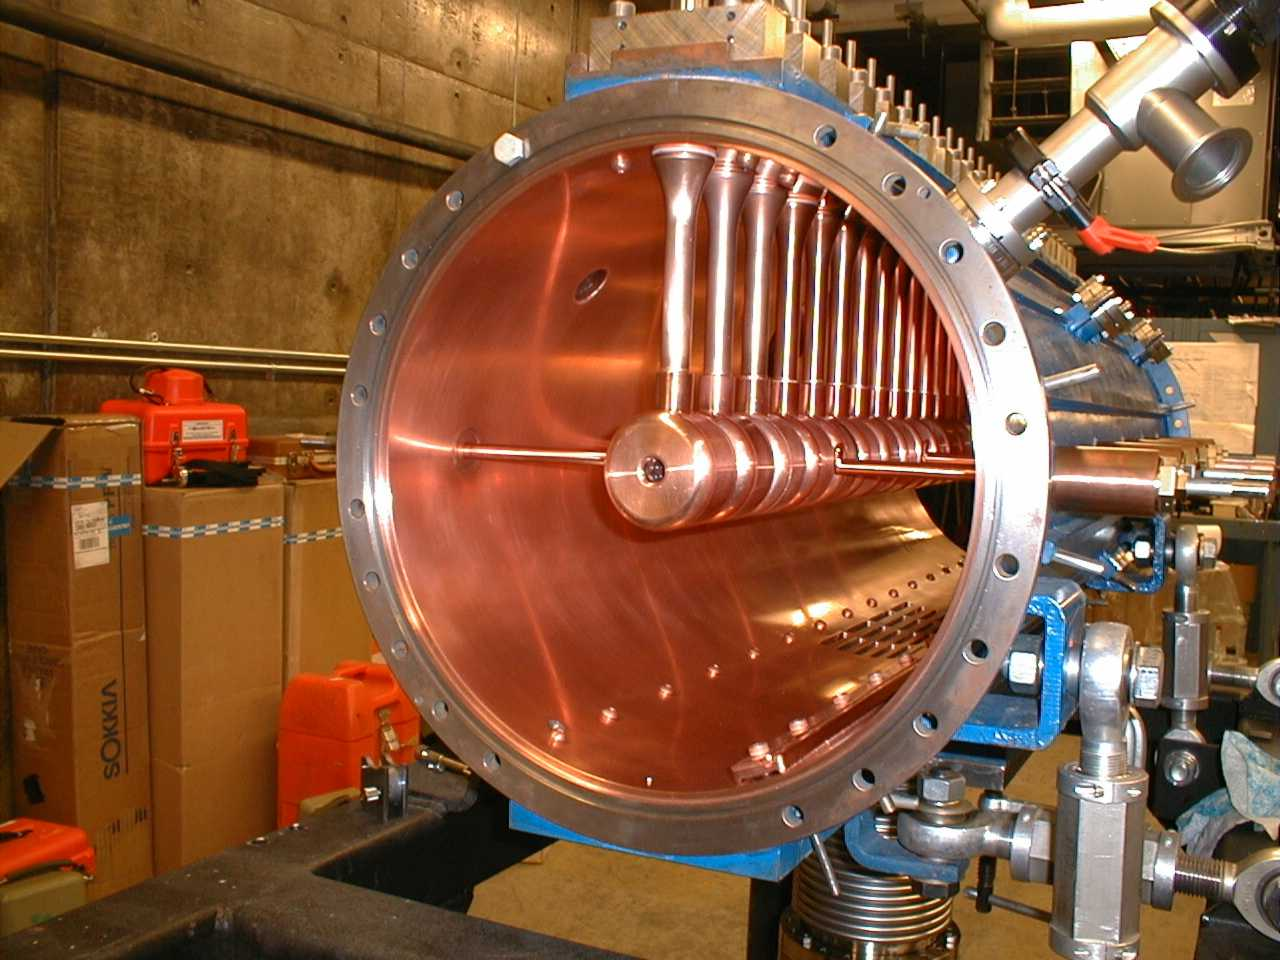
\includegraphics[width=\textwidth]{lineerhizlandirici}
    \caption{Doğrusal Hızlandırıcı}
  \end{minipage}
  \hfill
  \begin{minipage}[b]{0.4\textwidth}
    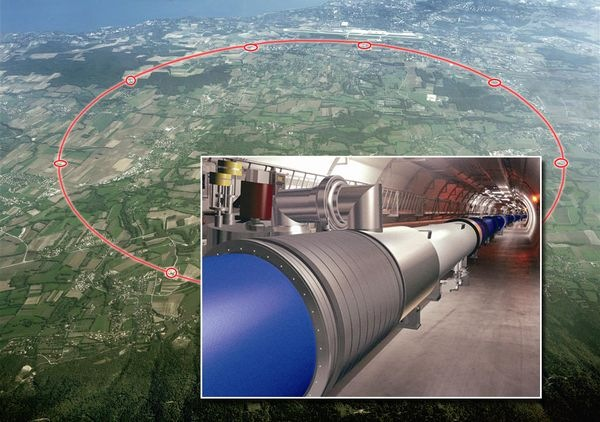
\includegraphics[width=\textwidth]{daireselhizlandirici}
    \caption{Dairesel hızlandırıcı}
  \end{minipage}
\end{figure}
\par Hızlandırıcı, bir mikroskop olarak düşünülebilir. Hızlandırıcıların en temel amaçlarından, maddenin temel yapı taşlarını ve aralarındaki etkileşmeleri incelemektir. Yüklü parçacıklar elektrik alanlar aracılığıyla hızlandırılırlar. Hızlandırılan bu parcaçıklar birbirlerine çapıştırılarak daha küçük parçacıkların ortaya çıkmasını sağlar. Ortaya çıkan bu parçacıklar dedektörlerle yükleri kütleleri ömürleri belirlenebilir. Hızlandırıcılar iki kısıma ayrılır. Bunlar doğrusal ve dairesel hızlandırıcılardır. Doğrusal Hızlandırıcılar; yüklü parçacıklar doğrusal yörüngelerde elektrostatik alanlar ve radyofrekans (RF) alanları ile hızlandırılırlar. Parçacıklar hızlandırılıp sabit hedefe çarptıktan sonra ışıma yapar. Sabit hedefe çarpma sonucunda yeni parçacıklar üretilir. \par
Dairesel hızlandırıcılar ; RF ile hızlandırılan ve manyetik alan ile yörüngede kalmasını sağlayan hızlandırıcılardır. Dünyadaki en büyük örneği ise Fransa-İsviçre sınırları içinde yer alan CERN'deki BHÇ'dir. \\





\section{Büyük Hadron Çarpıştırıcısı}
Büyük Hadron Çarpıştırıcısı'nın çevresi 27 km olup 100 m derinliktedir. BHÇ'de protonlar ilk olarak doğrusal hızlandırıcılarda belli bir enerji seviyesine çıkartılırlar. Daha sonra 1.4 GeV'lik itici bir enerji ile Proton Sinkrotronda 25 GeV ve Süper Proton Sinkrotronda 450 GeV'e çıkartılırlar ve BHÇ halkasına aktarılırlar. Yüksek enerjili bu protonları dairesel bir yol üzerinde tutmak için 1232 adet süperiletken mıknatıs kullanılmıştır. Bu hızdaki protonları dairesel bir yol üzerinde tutmak için gerekli olan manyetik alan ;
\begin{equation}
B= \frac{p}{q \cdot R{BHC}}
\end{equation}
ile hesaplanır. Burada $q$ protonun yükü, $p$ momentumları ve $R_{BHC}$ dedektörün yarıçapıdır.
\begin{figure}[!htbp]
\centering
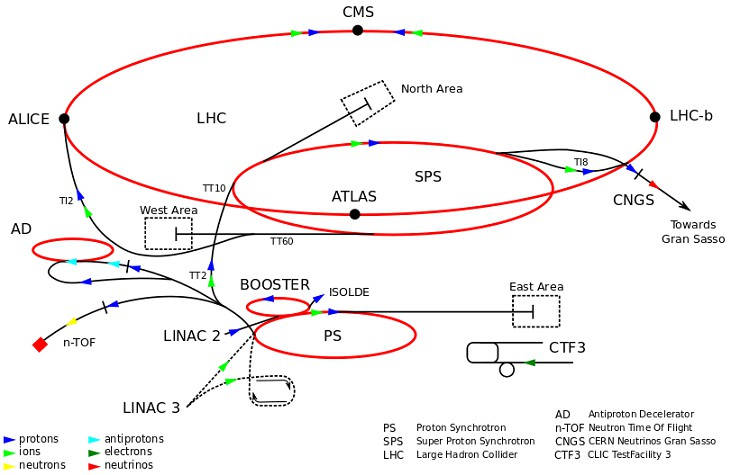
\includegraphics[scale=0.3]{CERN-accelerator-complex}
\caption{Büyük Hadron Çarpıştırıcısı}
\end{figure}
  ayrıca BHC'de protonlar demetler halinde gönderilirler ve 7 metre mesafe ile her demette $1.15 10^{11}$ adet proton bulunmaktadır.

Bu deneylerde bilinmesi gereken bazi kavramlar mevcuttur. Bunlardan ikisi kütle merkezi çerçevesi ve Luminosite önemli kavramlardandır.\\
\par Kütle merkezi çerçevesi : Bir sistemin hareketini çoğu kez, referans çerçevesinin orijinini kütle merkezinde ve durgun olarak incelemek uygun olur. Bu kütle merkezi çerçevesidir. Cern bu çerçevede iki ayrı proton demetinin kütle merkezi enerjisini $\sqrt{s}$ ile tanimlamistir. 2009 yıllarının sonunda Cern $\sqrt{s}=2.36 TeV$ lik carpışmalar gerceklestirirken. 19 Mart 2010 tarihinde $\sqrt{s}=3.5 TeV$ lik enerji ile çarpıştırmalar yaptı. Şu anda Cern $\sqrt{s}=14 TeV$ lik enerji ile çarpışmalardan veri toplamaktadir.
\begin{figure}[!htbp]
\centering
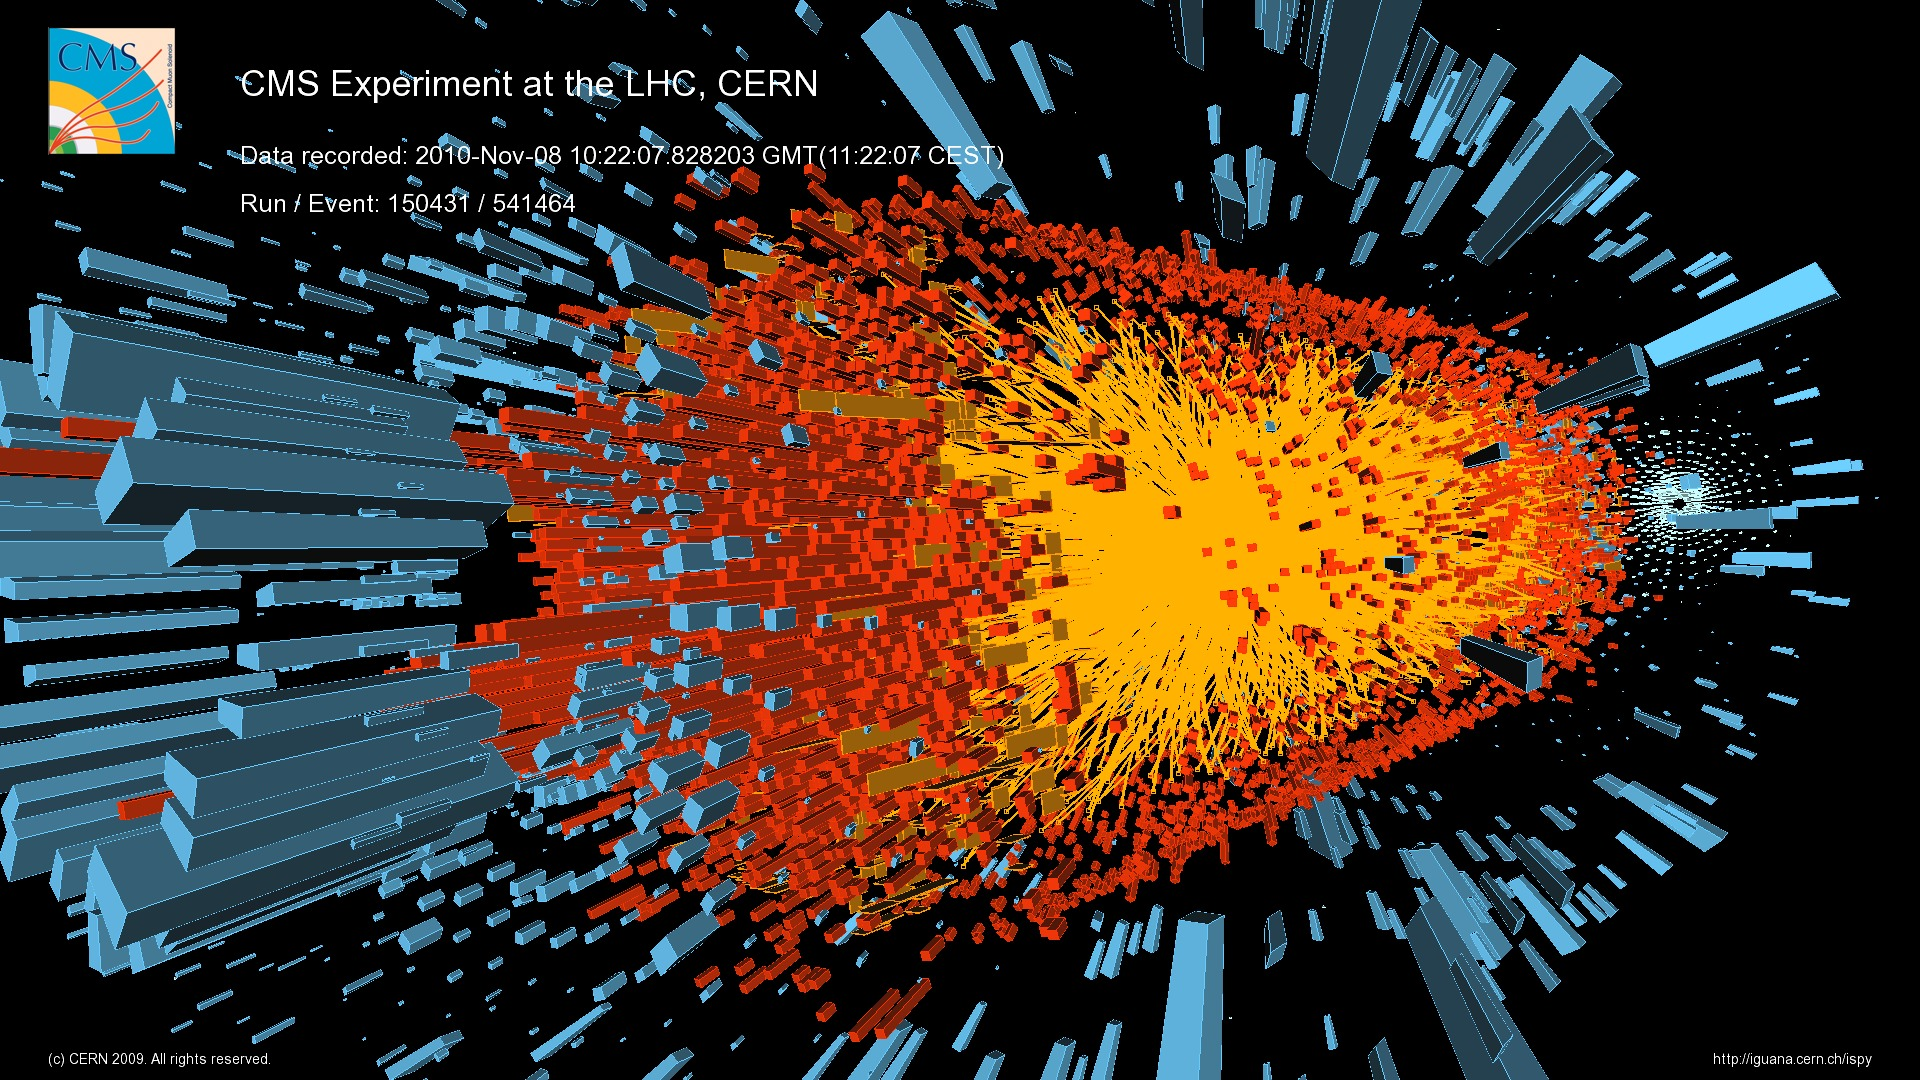
\includegraphics[scale=0.2]{carpisma}
\caption{CMS dedektorunde bir carpisma ve bu carpisma sonucu parcaciklarin dedektor uzerinde biraktigi izler}
\end{figure}

Luminosite : Işıklılık anlamına gelmektedir. Çarpıştırılan iki proton demetinin karşı karşıya gelme ihtimalini söyler. Luminositenin basit yaklaşımı;
\begin{equation}
L= \frac{f_c n_1 n_2}{A}
\end{equation}
$f_c$ proton demetinin çarpısma ihtimali $n_1$ ve $n_2$ proton demetlerinin icerisinde bulunan proton miktari ve $A$ ise proton demetinin enlemsel kesitidir. Diğer bir tanımı ise;

\begin{equation}\label{eq:liminosite}
\mathcal{L}=\frac{1}{\sigma} \frac{dN}{dt}
\end{equation}
\begin{equation} \label{eq:liminosite2}
\mathcal{L}_{int}=\int \mathcal{L} dt
\end{equation}
\par \ref{eq:liminosite} denkleminden görüldüğü üzere Liminosite birim zamandaki olay sayısı ile doğru orantılı ancak etkileşim içinde bulunduğu saçılma tesir kesiti ile ters orantılıdır. Denklem \ref{eq:liminosite2} ise belirli zaman aralığındaki integralidir. \ref{eq:liminosite} denklemini \ref{eq:liminosite2} yerine koyarsak;

\begin{equation}\label{eq:liminosite3}
\mathcal{L}_{int} = \frac{N}{\sigma}
\end{equation}
\ref{eq:liminosite3} denklemini elde ederiz. Yani bu iki kavram ile Luminosite değerinin büyük olması çarpışmanın o kadar fazla olacağı anlamına gelmektedir. Elimizde ne kadar fazla çarpışma varsa o kadar daha çok veri var demektir. Luminosite değerini arttırmak için $\sqrt{s}$'i arttırmamız gerekir. Böylece proton demetleri içerisindeki protonları arttırarak daha fazla veri üzerinde daha sağlıklı analizler gerçekleştirebiliriz.

\begin{figure}[!htbp]
\begin{center}
\label{pic:liminosite}
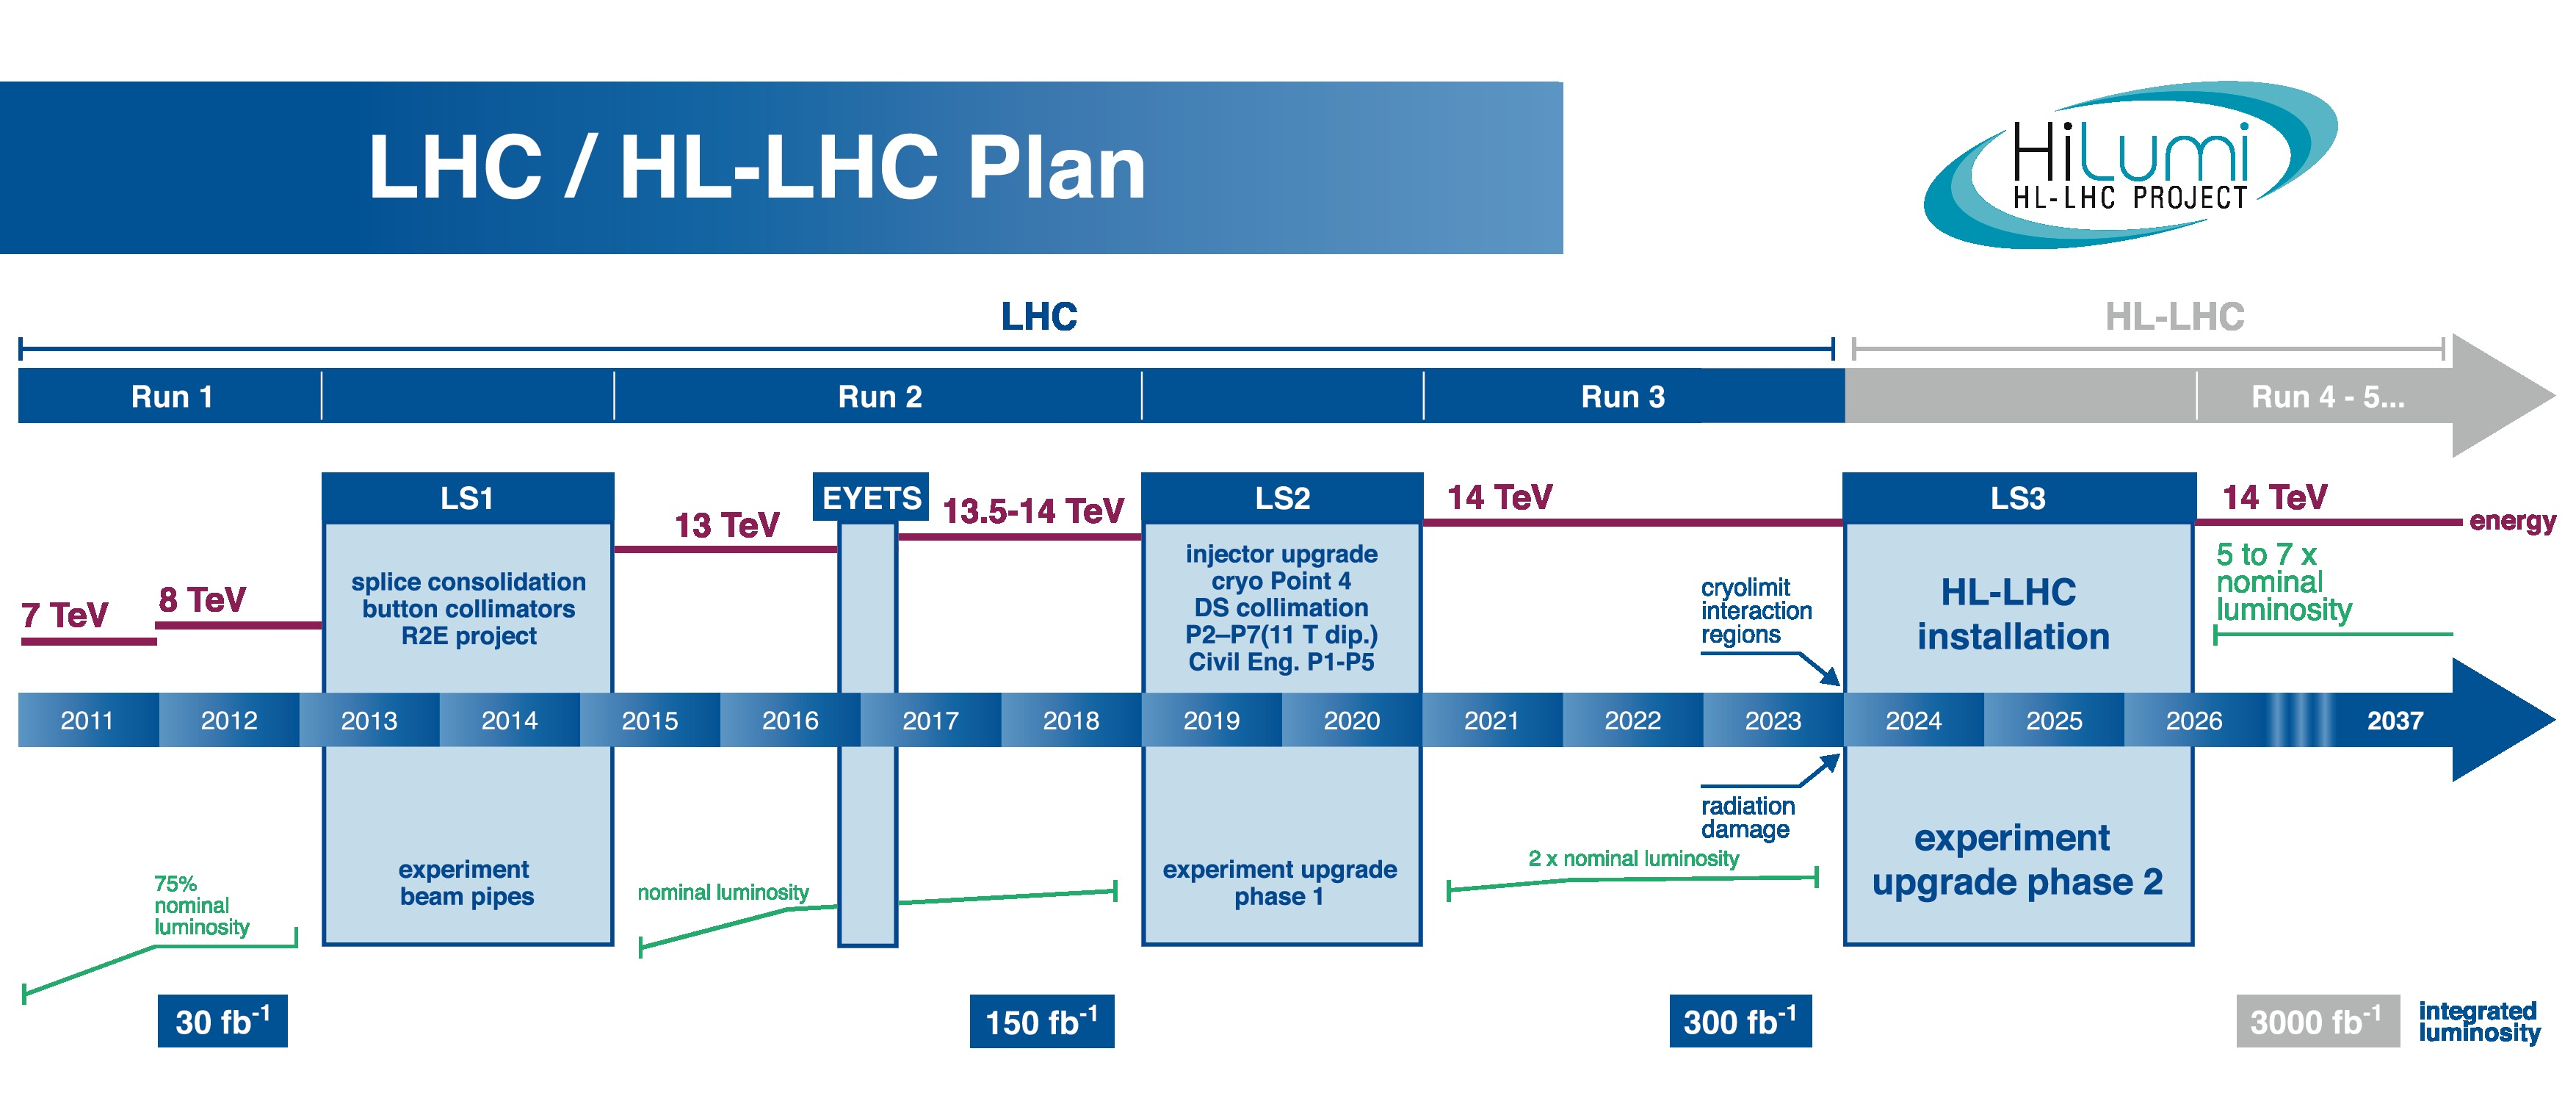
\includegraphics[scale=0.5]{HL-LHC-plan-2016-01}
\caption{Cern Integrated Liminosite}
\end{center}
\end{figure}
Yukarıda görüldüğü üzere Liminosite 2012 yılına kadar $30 fb^{-1}$ iken 2023 planlarında bu değerin 10 katına çıkmaktadır.
\par BHC üzerinde 4 büyük dedektör bulunmaktadir. Bunlar ; Büyük Toroidal Detektör (ATLAS), CMS, Büyük İyon Çarpıştırma Deneyi (ALICE) ve B fiziği araştırmaları yapan LHCb’dir.

\section{ATLAS}
ATLAS, 45 m uzunlukta, 25 m yükseklikte ve 7000 tonluk bir kütleye sahiptir. ATLAS dedektörü süpersimetrik parçacıkların ürünleri, ağır vektör bozonları, ekstra boyutlar ve Higgs bozonları gibi sınırsız çeşitlilikte fizik olaylarını incelemektedir.

%%%%%%%%%%%%%%%%%%%%%%%%%%%%%%%%%%%%%%%%%%%%%%%%%%%%%
\begin{figure}[!htbp]
        \centering
        \begin{subfigure}[b]{0.475\textwidth}
            \centering
            \includegraphics[width=\textwidth]{ATLAS_large}
            \caption[Atlas Dedektörü]%
            {{\small Atlas Dedektörü}}    
        \end{subfigure}
        \hfill
        \begin{subfigure}[b]{0.360\textwidth}  
            \centering 
            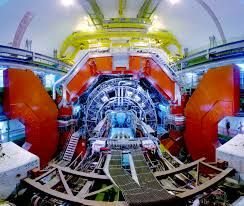
\includegraphics[width=\textwidth]{alice}
            \caption[Alice Dedektörü]%
            {{\small Alice Dedektörü}}    
        \end{subfigure}
        \vskip\baselineskip
        \begin{subfigure}[b]{0.475\textwidth}   
            \centering 
            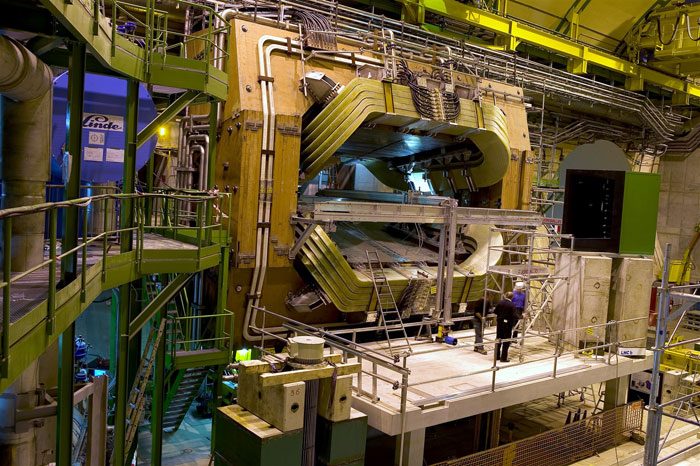
\includegraphics[width=\textwidth]{lhcb}
            \caption[LHCB]%
            {{\small LHCB}}    
        \end{subfigure}
        \caption[ CMS üzerindeki dedektörler]
        {\small CMS üzerindeki dedektörler} 
    \end{figure}



%%%%%%%%%%%%%%%%%%%%%%%%%%%%%%%%%%%%%%%%%%%%%%%%%%%%%%



\section{ALICE}
ALICE 16 m yüksekliğinde, 26 m uzunluğunda ve 10000 tonluk bir kütleye sahiptir. Burada çok küçük boyutlardaki maddenin fiziği araştırılmaktadır. Genel olarak bu deneyde çekirdek-çekirdek çarpışmaları ile quark-qluon plazma yapıları incelenmektedir.

\section{LHCb}
LHCb 21 m uzunluğunda, 10 m yüksekliğinde ve 5600 ton ağırlığındadır. b-quark ve B mezonlarin ozelliklerini ve parite bozunmasını araştırmak için dizayn edilmistir.

\section{CMS}
CMS 21.6 m uzunluğunda 14.6 m çapında ve 12500 ton ağırlığındadır. CMS'in merkezinde, 13 m uzunluğunda, 11.8 m iç çapında 4 T'lik süper iletken solenoid mıknatıslar bulunmaktadır. Çarpışmada meydana gelen yüklü parçacıkların izini belirlemek için en iç kısımda iz dedektörü bulunmaktadir. İz dedektörünün hemen arkasında elektronların ve fotonların enerjilerini ölçen elektromanyetik kalorimetre ve hemen ardından da kuvvetli etkileşen parçacıkları ölçmek için hadronik kalorimetre yer almaktadır. Son olarak en dışta muonların yük ve momentumlarını ölçmek için muon odacıkları bulunmaktadır. CMS dedektörü Higgs arayışı dahil SUSY gibi teorileri sınamak için veriler toplamaktadır.
\begin{figure}[!htbp]
\begin{center}
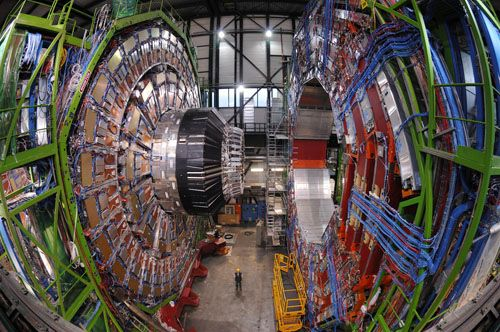
\includegraphics[scale=0.8]{cms}
\caption{CMS Dedektoru}
\end{center}
\end{figure}

\newpage
\subsection{CMS Koordinat Sistemi}
CMS'de kordinat sisteminin merkezi çarpışma noktası olarak seçilirse; x-ekseni ; radyal olarak BHC halkasının merkezine doğru yönelmiş, z-ekseni protonların geldiği yön ve son olarak y ekseni bu 2 eksene dik olan eksendir.xy ekseninde ölçülen azimut açısı $\phi$ yz düzleminde ölçülen açı $theta$ olmak üzere,CMS kutup açısı yerine psudorapidite $\eta$ ile $\theta$ arasında \ref{eq:eta}'daki gibi bir eşitlik bulunmaktadır. $\theta=0$ +z yönünü $\theta=\pi$ -z yönünü belirtmektedir.

\begin{equation} 
\eta = -\ln\left( \tan({\theta}/{2}) \right )
\label{eq:eta}
\end{equation}

\begin{figure}[!htbp]
\begin{center}
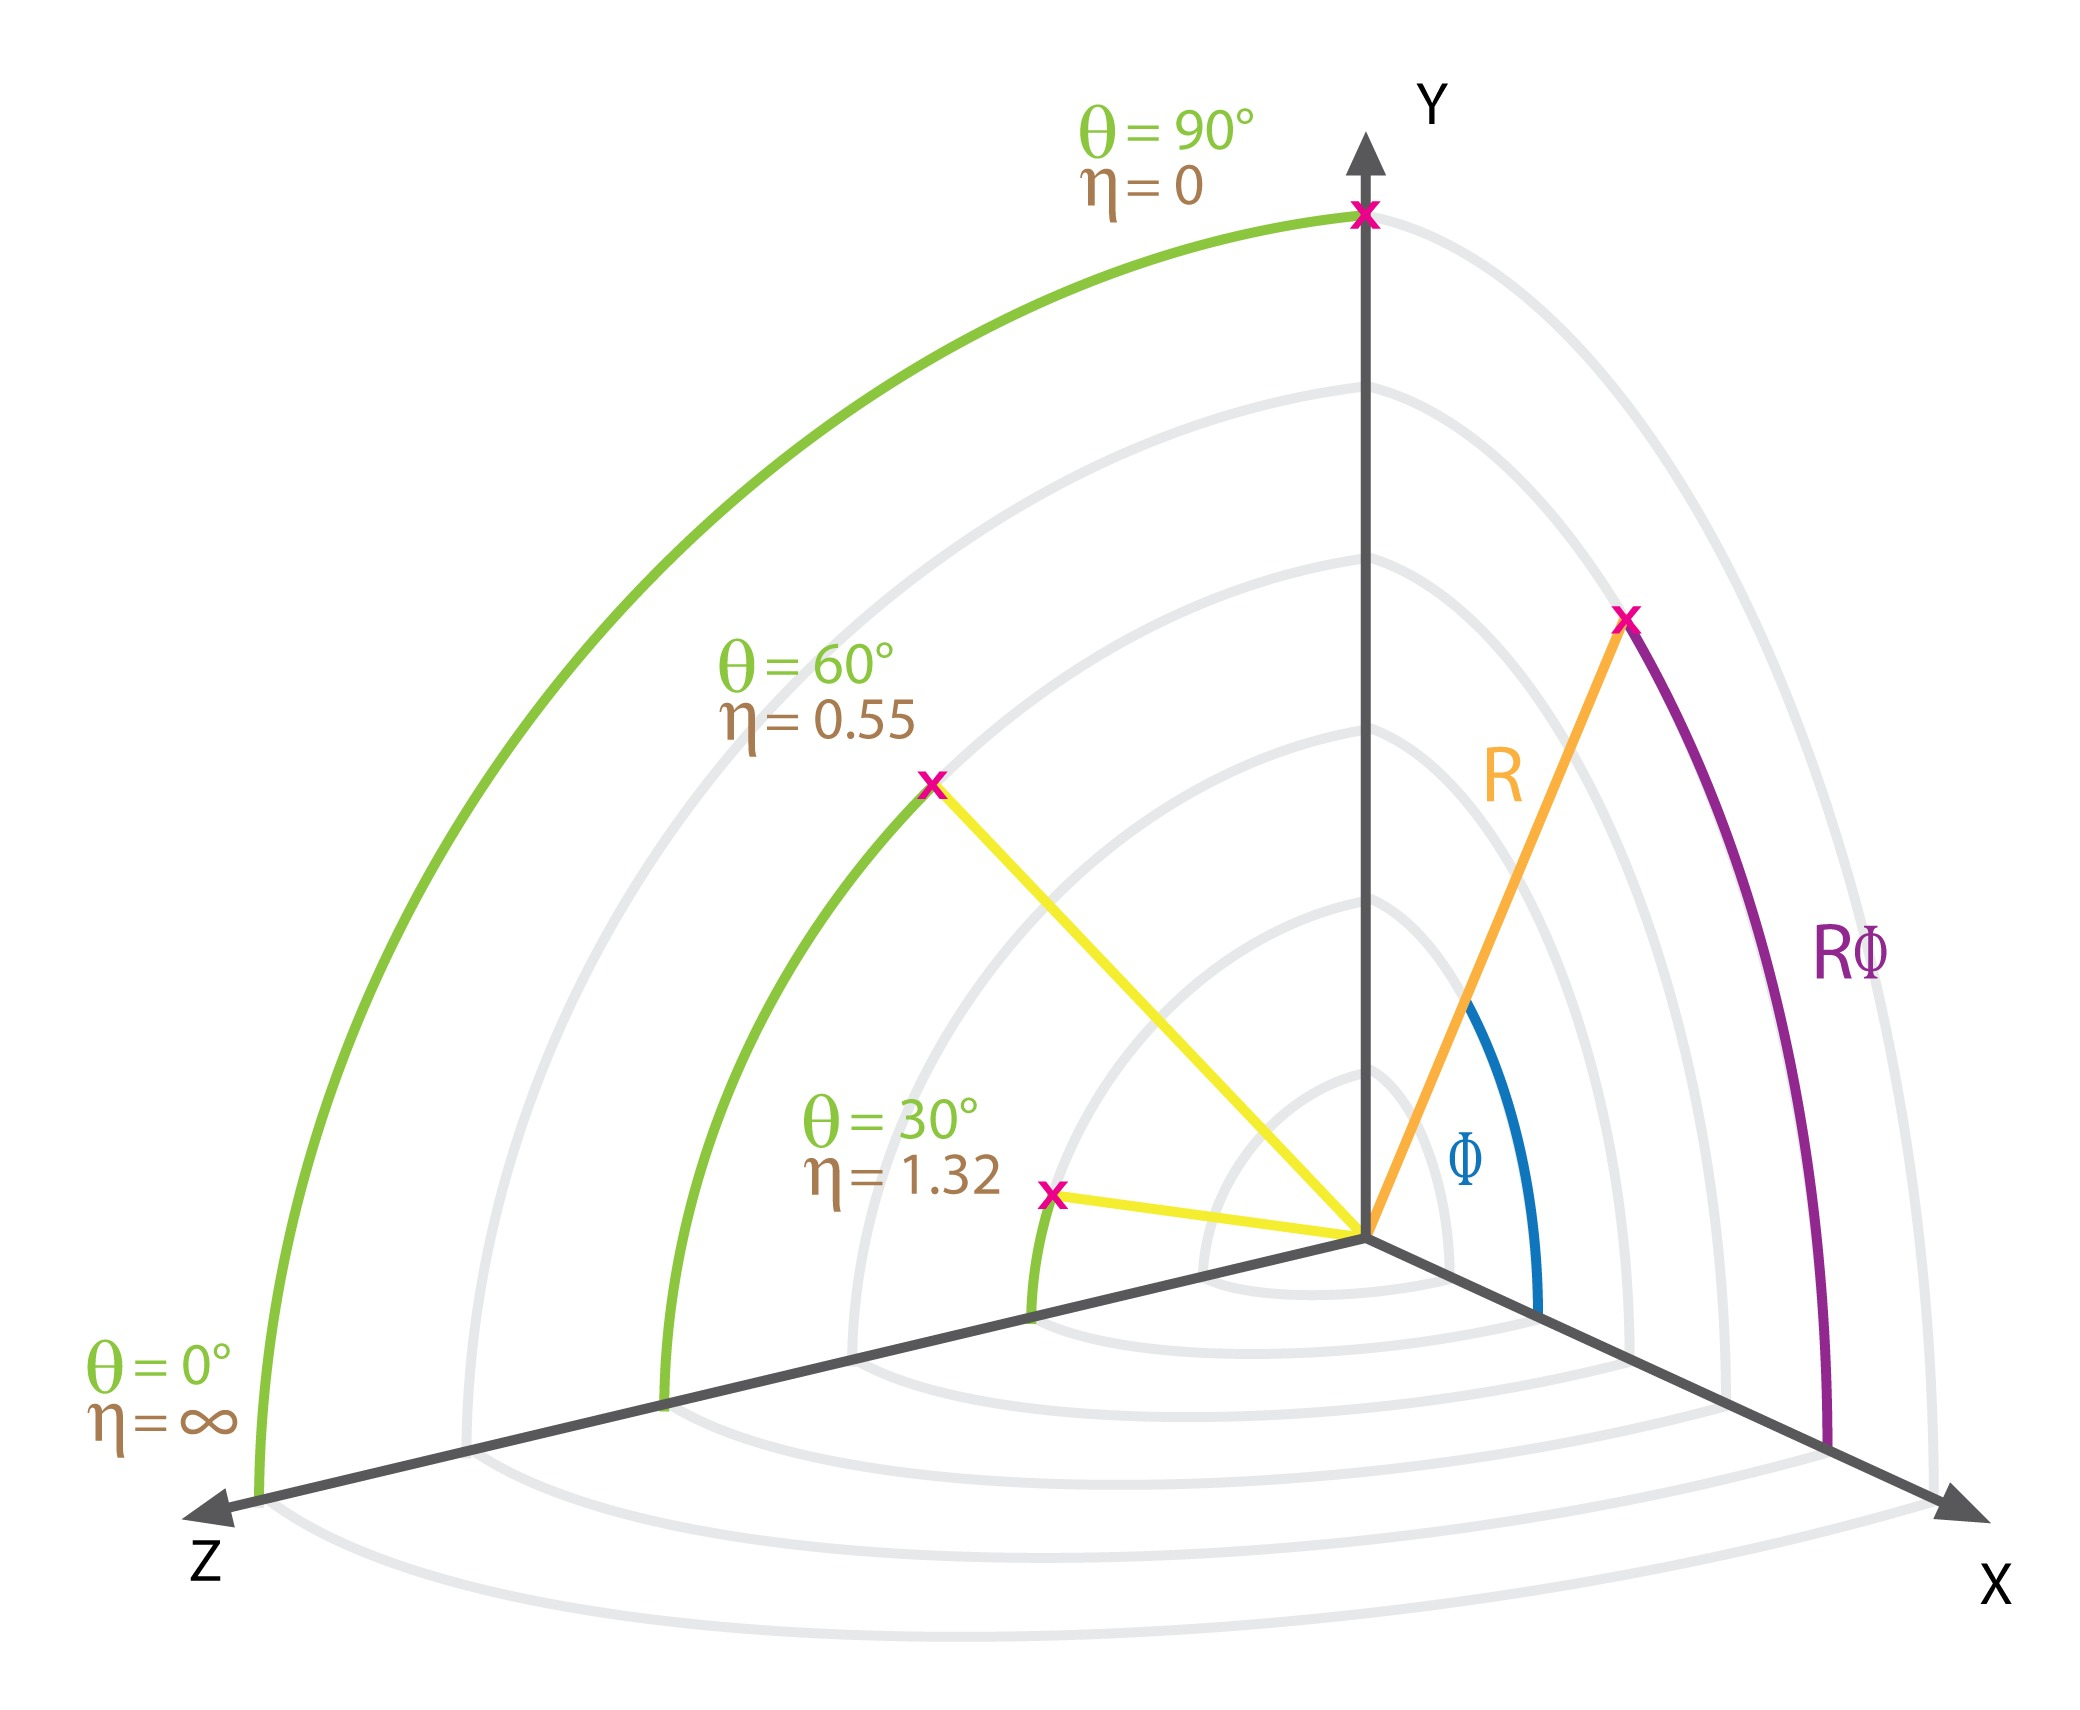
\includegraphics[scale=0.07]{img_cms_coordinates}
\caption{CMS Dedektoru koordinat sistemi}
\end{center}
\end{figure}

$\phi=0$ +x yonunde $\phi=\pi/2$ +y yonunu gostermektedir ve $phi$,$-\pi$ ile $+\pi$ arasinda degerler alabilir. Acisal uzaklik $\triangle R$ \ref{eq:daltar} seklinde $\phi$ ve $\eta$ cinsinden ifade edilebilir.

\begin{equation}
\triangle R = \sqrt{(\triangle \phi)^2 + (\triangle  \eta)^2}
\label{eq:daltar}
\end{equation}


\subsection{CMS'in Alt Dedektorleri}

Silindirik bir yapıya sahip olan CMS dedektörü içten dışa doğru İz	dedektörü(beam-line ı çevreler), ECAL\footnote{Elektromanyetik Kalorimetre}, HCAL\footnote{Hadronik Kalorimetre} ve Muon dedektörüne sahiptir.
\begin{figure}[!htbp]
\begin{center}
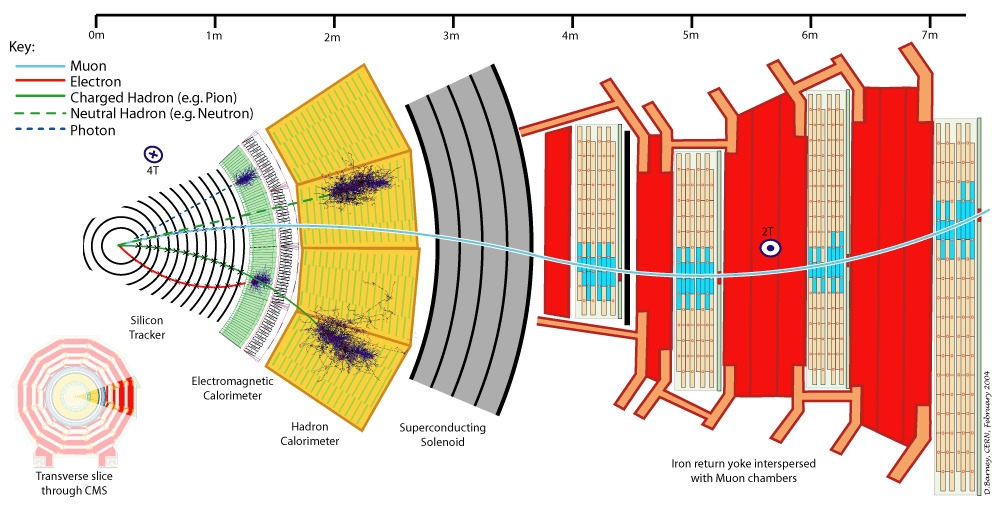
\includegraphics[scale=0.3]{CMS_Slice}
\caption{CMS alt dedektorleri}
\end{center}
\end{figure}
\begin{enumerate}


\item \textbf{İz Dedektoru}
Bu dedektörün çalışma mantığı çarpısmada oluşan yüklü parçacıkların enerkilerinin bir kısmını iyonizasyonla kaybettirerek parçacıkların mentumunun, yükünün ve törüngesinin belirlenmesini sağlar.$-2.5 < \eta < 2.5 $ psudorapidite aralığında yer alır ve parçacıkların bıraktıkları izleri belirler. İz dedektörleri piksel dedektör ve iç izleyici olarak 2 sınıfa ayrılır. 

\textbf{Piksel Dedektör}
Çarpışma noktasına en yakın olan elemanıdır. Bu dedektör ağır ve kısa ömürlü parçacıklar ile yapısında b-quark bulunan hadronların bozulmasıyla oluşabilecek birincil ve ikincil etkileşim noktalarının belirlenmesini sağlar.
\textbf{İç İzleyici Sistem}
Etkileşme noktasına yakın olan 3 katmanlı hibrit piksel dedektöre sahiptir. Bu sistem yüksek luminositede ve çaplardaki yüklü parçacıklara göre yakın orta ve dış bölge olarak ayrılır.
\item \textbf{Elektromanyetik Kalorimetre}
Bu dedektör, fotonlar ve pozitronları ölçmek için tasarlanmıştır. İçerisinde 61200 adet $(PbWO_4)$ kristali bulunmaktadır. Elektromanyatik kalorimetre hadronik kalorimetre ile Jet lerin ölçülmesini sağlar.
\item \textbf{Hadronik Kalorimetre}
HCAL CMS'de manyetik halka içindeki son kısımda bulunan dedektördür. HCAL çarpışmadan çıkan parçacıkların kayıp enerjilerini ve en önemlisi jetleri ölçen dedektördür. HCAL $|\eta| \leq 5.0 $ aralığını kapsamaktadır. HCAL'da odacıklar $\eta$ ve $\phi$'ye göre yerleştirilirler. Bu odacıklardaki değişikliklerle çıkan Jet'lerin Enerjileri ve yönelimleri belirlenmektedir.
\item \textbf{Müon Sistemi}
Muon sistemi dedektörün en dış kısmında bulunmaktadır. Amacı muonları tespit etmektir. Muon sistemindeki disklerin her biri $\phi = 30 $ dereceye karşılık gelen 12 sektöre ayrılmıştır. 
\end{enumerate}